\subsection{Minimum/Maximum Momentum cuts}
\label{pCuts}
A study \cite{cnKEgiyan} of the inclusive cross section at various beam energies in CLAS developed a parametrization of the low momentum cut $p_{min}$ as a function of the calorimeter low trigger %total energy
threshold (in milli-Volts)% % of the trigger discriminator:

\begin{equation}
\label{ecThres}
p_{min} \text{ (MeV)} = 214 + 2.47\times EC_{threshold} \text{ (mV)}
\end{equation}

The low threshold for EC-total energy for EG4 was 65 mV \cite{eg4Hm_wb}, so, %therefore, %GED
the minimum momentum cut was determined to be at:  $p_{min} = 0.37 \approx 0.4$  GeV. In addition, %On top of this, 
another minimum cut of $p_{min}=0.2*E_{beam}$ was added, so the actual minimum cut amounted to the larger of those two. %whichever was bigger between 0.4 GeV and  20\% of the beam energy. %\textbf{\textcolor{red}{Comment: Reason for 0.2*Eb cut to be explained later}}
Likewise, the momentum cannot be more than that of the %transferred by the beam and the maximum possible momentum that can be transferred is equal to the 
beam energy (in natural units), therefore, the upper %or maximum 
cut on the momentum is: $p_{max}=E_{beam}$.

Figure \ref{pMnMxCt} shows the momentum distribution of the electron candidates for the 2 GeV data and the minimum and maximum cuts.


\begin{figure}[H]%[hp] %ht, htpb (p - float, b = bottom, h=? t = top)
\centering
%\leavevmode 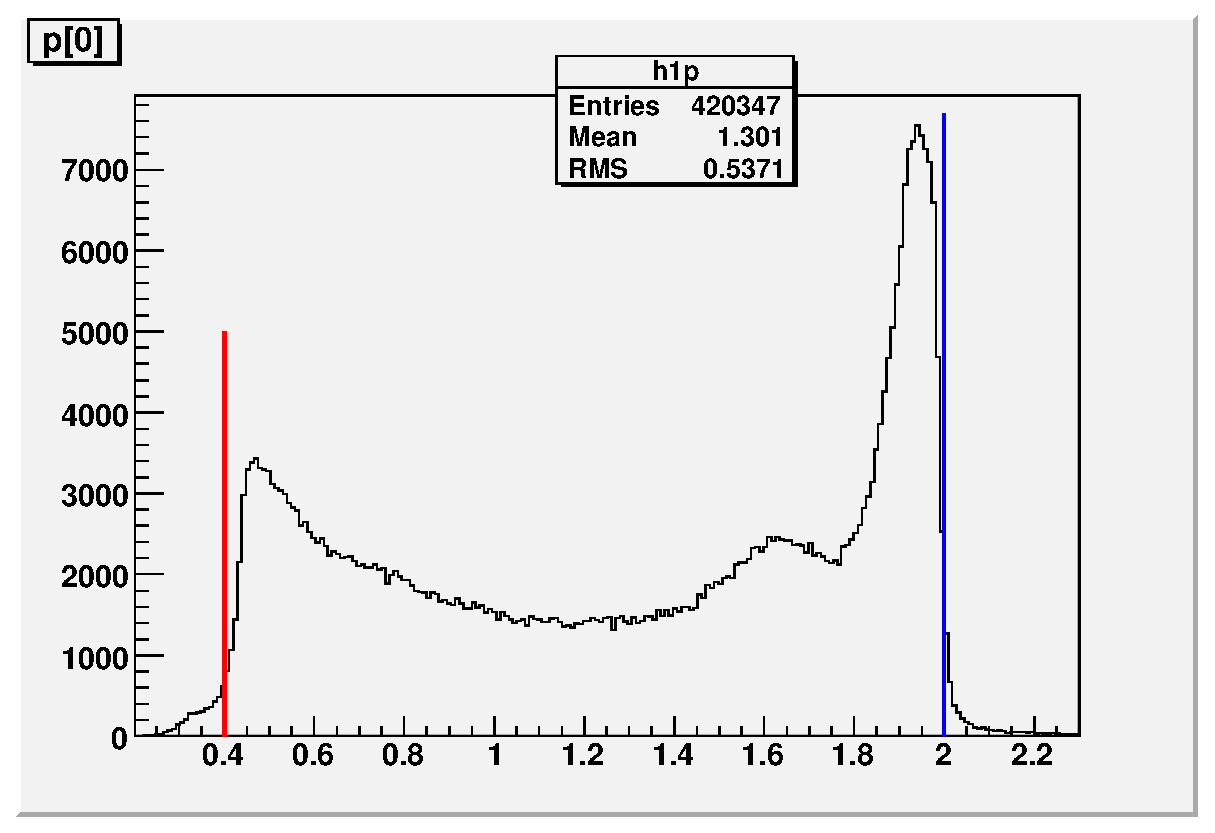
\includegraphics[width=0.8\textwidth]{TexmakerMyFinTh/chap4simul/FigCuts/pMinCtFrmRtPrmptEb2.eps}  %0.6 is the fraction of the real image width????
\leavevmode 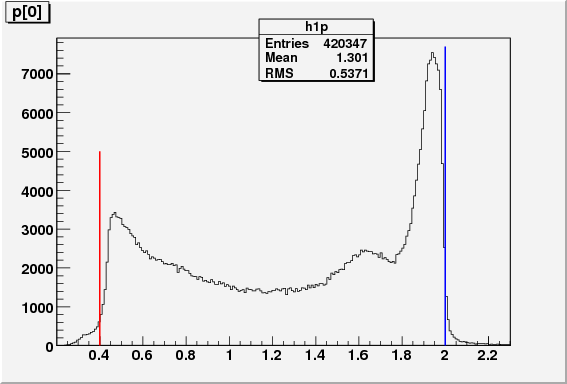
\includegraphics[width=0.8\textwidth]{TexmakerMyFinTh/chap4simul/FigCuts/pMinCtFrmRtPrmptEb2}  %0.6 is the fraction of the real image width????
\caption[Maximum and minimum momentum cuts]{The maximumum and minimum momentum cuts (on 2.0 GeV \nd3 data).
%\textcolor{red}{SEK: Memo to self: in the future use 0.45 GeV.}
}
\label{pMnMxCt}
\end{figure}
